%%% The main file. It contains definitions of basic parameters and includes all other parts.

% Meta-data of your thesis (please edit)
\input metadata.tex

% Generate metadata in XMP format for use by the pdfx package
\input xmp.tex

%% Settings for single-side (simplex) printing
% Margins: left 40mm, right 25mm, top and bottom 25mm
% (but beware, LaTeX adds 1in=25.4mm implicitly)
\documentclass[12pt,a4paper]{report}
\setlength\textwidth{145mm}
\setlength\textheight{247mm}
\setlength\oddsidemargin{14.6mm}
\setlength\evensidemargin{14.6mm}
\setlength\topmargin{0mm}
\setlength\headsep{0mm}
\setlength\headheight{0mm}
\setlength{\emergencystretch}{3em}
% \openright makes the following text appear on a right-hand page
\let\openright=\clearpage

%% Settings for two-sided (duplex) printing
% \documentclass[12pt,a4paper,twoside,openright]{report}
% \setlength\textwidth{145mm}
% \setlength\textheight{247mm}
% \setlength\oddsidemargin{14.6mm}
% \setlength\evensidemargin{0mm}
% \setlength\topmargin{0mm}
% \setlength\headsep{0mm}
% \setlength\headheight{0mm}
% \let\openright=\cleardoublepage

%% If the thesis has no printed version, symmetric margins look better
% \documentclass[12pt,a4paper]{report}
% \setlength\textwidth{145mm}
% \setlength\textheight{247mm}
% \setlength\oddsidemargin{7.1mm}
% \setlength\evensidemargin{7.1mm}
% \setlength\topmargin{0mm}
% \setlength\headsep{0mm}
% \setlength\headheight{0mm}
% \let\openright=\clearpage

%% Generate PDF/A-2u
\usepackage[a-2u]{pdfx}

%% Prefer Latin Modern fonts
\usepackage{lmodern}
% If we are not using LuaTeX, we need to set up character encoding:
\usepackage{iftex}
\ifpdftex
\usepackage[utf8]{inputenc}
\usepackage[T1]{fontenc}
\usepackage{textcomp}
\fi

%% Further useful packages (included in most LaTeX distributions)
\usepackage{amsmath}        % extensions for typesetting of math
\usepackage{amsfonts}       % math fonts
\usepackage{amsthm}         % theorems, definitions, etc.
\usepackage{bm}             % boldface symbols (\bm)
\usepackage{booktabs}       % improved horizontal lines in tables
\usepackage{caption}        % custom captions of floating objects
\usepackage{dcolumn}        % improved alignment of table columns
\usepackage{floatrow}       % custom float environments
\usepackage{graphicx}       % embedding of pictures
\usepackage{indentfirst}    % indent the first paragraph of a chapter
\usepackage[nopatch=item]{microtype}   % micro-typographic refinement
\usepackage{paralist}       % improved enumerate and itemize
\usepackage[nottoc]{tocbibind} % makes sure that bibliography and the lists
			    % of figures/tables are included in the table
			    % of contents
\usepackage{xcolor}         % typesetting in color
\usepackage[dvipsnames]{xcolor}

% The hyperref package for clickable links in PDF and also for storing
% metadata to PDF (including the table of contents).
% Most settings are pre-set by the pdfx package.
\hypersetup{unicode}
\hypersetup{breaklinks=true}

% Packages for computer science theses
\usepackage{algpseudocode}  % part of algorithmicx package
\usepackage{algorithm}
\usepackage{fancyvrb}       % improved verbatim environment
\usepackage{listings}       % pretty-printer of source code

% You might want to use cleveref for references
% \usepackage{cleveref}

% Set up formatting of bibliography (references to literature)
% Details can be adjusted in macros.tex.
%
% BEWARE: Different fields of research and different university departments
% have their own customs regarding bibliography. Consult the bibliography
% format with your supervisor.
%
% The basic format according to the ISO 690 standard with numbered references
\usepackage[natbib,style=iso-numeric,sorting=none]{biblatex}
% ISO 690 with alphanumeric references (abbreviations of authors' names)
%\usepackage[natbib,style=iso-alphabetic]{biblatex}
% ISO 690 with references Author (year)
%\usepackage[natbib,style=iso-authoryear]{biblatex}
%
% Some fields of research prefer a simple format with numbered references
% (sorting=none tells that bibliography should be listed in citation order)
%\usepackage[natbib,style=numeric,sorting=none]{biblatex}
% Numbered references, but [1,2,3,4,5] is compressed to [1-5]
%\usepackage[natbib,style=numeric-comp,sorting=none]{biblatex}
% A simple format with alphanumeric references:
%\usepackage[natbib,style=alphabetic]{biblatex}

% Load the file with bibliography entries
\addbibresource{bibliography.bib}

% Our definitions of macros (see description inside)
\input macros.tex

%%% Title page and various mandatory informational pages
\begin{document}
\include{title}

%%% A page with automatically generated table of contents of the thesis

\tableofcontents

%%% Each chapter is kept in a separate file
\chapter*{Introduction}
\addcontentsline{toc}{chapter}{Introduction}

Arduino is a very popular microcomputer among amateurs and professionals alike. Despite this, testing the code for an Arduino machine can be fairly difficult. Debugging options are limited and the user needs to rely on additional measuring equipment. The usual choice is to test the code with an AVR emulator. Emulation is the process of running machine code on a hardware that doesn't match its instruction set. AVR is the processor that controls the Arduino board. These emulators are sometimes part of a bigger logical circuit simulation system, other times they are just a single piece of software.

Goal of this work is to skip the emulation process and create a working Arduino simulator by mimicking the changes of digital values on the board's pinout. The user code will be compiled directly to the x86-64 architecture instruction set, which is our target platform, and thus able to run at the native speed of the host machine.

Bundled with this simulator is a graphic application for creating and testing logical circuits. This GUI is written with Avalonia framework and will contain Arduino as it's main component. The point of this application is to attach to the running Arduino simulator and visualize the expected Arduino behavior with user's code on a given circuit. We want to give the user the power to compose their own circuits, and define the behavior and looks of their components. Additionally, the user will be able to debug their program, while the GUI is running, using their preferred IDE and C++ debugger, providing real-time feedback and inspection when stepping through the code.

\subsubsection{Structure of the thesis}

This thesis starts with a brief introduction of technologies we've chosen for achieving our vision from the introduction. Then we lay down very specific goals and requirements, we want to address in this very thesis, using the mentioned technologies. In chapter \ref{ch:arduino} we introduce the reader to programming for Arduino boards. We show what is required from Arduino programs (\ref{sec:sketches}), how they access the board's I/O (\ref{sec:arduino_io}), and how are they built (\ref{sec:arduino_build}).

In chapter \ref{ch:architecture} we provide a high level look on the core systems of the work. We show why it is required to split the work into 2 applications (or more accurately processes) and we expose the reader to the world of inter-process communication (\ref{sec:ipc}). We show how it can be achieved using TCP connection (\ref{subsec:ipc_tcp}), shared memory (\ref{subsec:ipc_shmem}) and events (\ref{subsec:events}), and what kind of problems had to be taken into consideration (\ref{subsec:ipc_considerations}). Then we delve into more details on how the individual projects and classes have been implemented in chapters \ref{ch:backend} and \ref{ch:frontend}.

Finally, the chapter \ref{ch:docs} consists of specifics on how to simulate Arduino code using the applications we developed for this thesis (\ref{sec:usage}). We specify how to create custom components and scenes for the circuit simulator (\ref{sec:component_spec}). And in the very end, we specify what interprocess communication protocols we have created for interacting with the simulator's backend, so that any other user interface can potentially be connected to it (\ref{sec:ipc_spec}).

\section{Technologies used}

\subsubsection{C++, CMake, Boost}

For technical reasons described in the subsection \ref{subsec:ipc_considerations}, the work is split into two processes: the frontend and the backend. The backend is written in C++, as it is almost identical to the language used for Arduino sketches (see \ref{sec:arduino_build}). This makes the build process of the user's code much simpler. In the C++ project we use Boost libraries that provide useful abstractions for communicating with other processes (\texttt{asio}, \texttt{interprocess}) and parsing command line arguments (\texttt{program\_options}). We use CMake as our metabuild system of choice, as it is the one we are the most familiar with.

\subsubsection{C\#}
 
The frontend is written in C\# from the .NET 9 Software development kit. We consider the language to be more convenient for writing many of the essential systems than its C++ counterpart. That includes handling the graphics, the user interactions, reflection and parsing numerous configuration files. We also believe the language will be more comfortable for users that wish to extend the simulator with their own components. Libraries are also much easier to set up and compile thanks to NuGet.

\subsubsection{Avalonia UI}

For the GUI we decided to use Avalonia UI. Avalonia is a popular open-source cross-platform .NET framework, used by major companies like JetBrains or Unity. It is based on the Microsoft's WPF framework utilising the same XAML markup language and many of the same core principles. We chose it specifically because neither WPF or its cross-platform successor MAUI are available on Linux, one of our target platforms.

\subsubsection{SVG}

We want to render the circuit's components using vector graphics, as they don't have a limited resolution. This is crucial, since we also want to render the components in different sizes and under different zoom levels. The most common file format for vector graphics is SVG, so this is the format we will require to be supplied for custom components. Avalonia provides a sufficient support for rendering vector graphics using the Skia engine under the hood, as all of its built-in controls are rendered with it.

\section{Specific goals of the thesis} \label{sec:goals}

\subsubsection{Target platforms:}
\begin{itemize}
    \item Linux (x86-64)
    \item Windows 10 or higher (64-bit)
\end{itemize}

\subsubsection{Software prerequisites:} \label{prerequisits}
\begin{itemize}
    \item arduino-cli \footnote{See section \ref{sec:arduino_build}}
    \item Minimal system requirements of Avalonia UI \footnote{See \url{https://docs.avaloniaui.net/docs/supported-platforms}}
    \item .NET 9 SDK or higher
    \item C++ compiler
    \item CMake
    \item C++ Boost libraries:
    \begin{itemize}
        \item asio
        \item interprocess
        \item program\_options
    \end{itemize}
\end{itemize}

\subsubsection{Simulator functional requirements}
\begin{itemize}
    \item Defines platform independent constants and macros from \texttt{Arduino.h}.
    \item Implements \texttt{digitalWrite}, \texttt{digitalRead}, \texttt{pinMode} and \texttt{millis} functions from \texttt{Arduino.h}.
    \item Declares and calls \texttt{setup} and \texttt{loop} functions with the behavior expected on an Arduino machine. 
    \footnote{The significance of the mentioned functions is described in detail in the chapter \ref{ch:arduino}}
    \item Compiles and runs any valid \texttt{Arduino UNO R3 SMD} sketch, preprocessed with the \texttt{arduino-cli} tool, containing only symbols mentioned above.
    \item Reflects behavior of the above functions in an internal Arduino state. Logs changes of this state in a text file.
    \item Integrates an interprocess communication mechanism for exchanging data with an external GUI application.
    \item The events incoming from a GUI application must be resolved in a manner, that preserves the continuity of events.
\end{itemize}

\subsubsection{GUI functional requirements}
\begin{itemize}
    \item The application must stay responsive during debugging of the simulator process.
    \item The application must be able to connect to the interprocess mechanism of the simulator.
    \item Simulates simplified digital circuits. Exact physical properties, like voltages and currents might not be implemented.
    \item Implements mechanism for defining custom components and visuals with \texttt{.yaml}, \texttt{.cs} and \texttt{.svg} files. These components include interactive controls, such as buttons.
    \item Implements mechanism for defining a circuit (scene) using the custom components.
    \item Predefines LED, button, voltage source and Arduino components, and a scene which utilizes these components.
    \item The changes to the simulator's internal state must be immediately reflected on visual components connected to the Arduino in the scene.
    \item The scene is able to be zoomed and panned. The visuals of the components must be rendered using vector graphics.
    \item Multiple interactable components may be pressed at once.
\end{itemize}
\chapter{Introduction to Arduino programming} \label{ch:arduino}

\section{Sketches}

The Arduino programs are commonly referred to as \textit{sketches}. A sketch is not a single file, but an entire directory, usually populated by files with the \texttt{.ino} extension, contaning the source code of the program. \texttt{.cpp}, \texttt{.c}, \texttt{.S} (assembly files), and header files like \texttt{.h} are also accepted as files contaning source code. Every sketch must contain a \texttt{.ino} file with a file name matching the sketch root directory name \cite{arduino_sketch_specs}.

The Arduino programming language, in which \texttt{.ino} files are written, is a C++ dialect with very subtle differences, mostly concerning linking of files and ommitting function declarations. Bodies of function definitions and variable declarations can be considered as a perfectly valid C/C++ code. 

The essential functions that an Arduino programmer has to define in their sketch are \texttt{void setup()} and \texttt{void loop()}. The \texttt{setup()} function is called once, when the program is booted. That is when the Arduino board is powered up, the program is uploaded to it, or when the reset button is pressed. The \texttt{loop()} function is called in a loop indefinitely. This is the proper place to define any interactions with the board, detecting inputs, updating timers, etc.

\section{Arduino board interface}

The target board \texttt{Arduino Uno R3 SMD} provides 6 analog and 14 digital general purpose pins, some of which can be used for I2C and SPI protocol communication, or PWM modulation. The most simple to use and simulate are the digital pins for general purpose I/O, so this thesis focuses exlucively on using these pins as such. \cite{arduino_r3_smd_specs}

The digital pins can be manipulated using only these 3 functions:
\begin{description}
    \item[\texttt{void pinMode(pin, mode)}] configures specified pin either as an input or an output
    \item[\texttt{value digitalRead(pin)}] reads the voltage on the pin, stores it as a digital value, either 1 or 0
    \item[\texttt{void digitalWrite(pin, value)}] when set to output, sets the voltage of the pin to corresponding value.
\end{description}

Pins are identified by their integer index. \texttt{mode} and \texttt{value}'s underlying type is also an integer, but it is preferred to use predefined constants, such as \texttt{INPUT}/\texttt{OUTPUT}, \texttt{HIGH}/\texttt{LOW} and such. Below is an example of a sketch from the Arduino's documentation, using only the described functions:

\begin{lstlisting}[language=csharp, caption=Sketch example \cite{arduino_digital_read}]
int ledPin = 13;  // LED connected to digital pin 13
int inPin = 7;    // pushbutton connected to digital pin 7
int val = LOW;    // variable to store the read value

void #setup#() {
  #pinMode#(ledPin, OUTPUT);  // sets the digital pin 13 as output
  #pinMode#(inPin, INPUT);    // sets the digital pin 7 as input
}

void #loop#() {
  val = #digitalRead#(inPin);   // read the input pin
  #digitalWrite#(ledPin, val);  // sets LED to the button's value
}
\end{lstlisting}

\section{Build process}

Before the code is compiled, all \texttt{.ino} go through a simple preprocessing stage. \texttt{\#line} directives are added. These link to the original line and file, when the code is debugged. All files are concatenated together, function declarations are generated at the top, and the \texttt{Arduino.h} is included. This header file is crucial as it declares the \texttt{void} and \texttt{loop} functions, functions for manipulating pins, common constants and mathematical functions, etc. At this point the sketch becomes a complete C++ source code.

It is also at this where we steer away from the standard compilation process, and apply our own \texttt{Arduino.h} implementation in our simulator. Usually, the C++ code would be linked to an implementation that contains binaries and constants for the given microchip installed on the target board. Then it would be compiled with a compiler for the given instruction set (e.g. \texttt{avr-gcc}). The code would be then transmitted over USB to the user's Arduino \cite{arduino_sketch_build}.

In our case, we include the entire preprocessed sketch in our simulator project written in C++, and compile it as whole for the instruction set of the host machine. This executable will implement mock functions declared in the \texttt{Arduino.h}, arduino's internal state, and a way to communicate the change of state to an external GUI application.

The entire process from preprocessing to compilation, can be orchestrated with the use of \texttt{arduino-cli} command line application. We will use it to preprocess the \texttt{.ino} for us, so that we end up with a clean C++ file we can include in our project. 

\chapter{Architecture design} \label{ch:architecture}

\section{Architecture overview}

The whole project is divided into two main parts. The purpose of the backend is to execute the Arduino code and simulate the change on the board's pinout. The purpose of the frontend is to reflect these changes on a user defined logical circuit, while offering the user control over the simulation. We chose to implement the backend in C++ and the frontend in C\#. Both backend and frontend are running in its own separate process.

\begin{figure}[ht]
    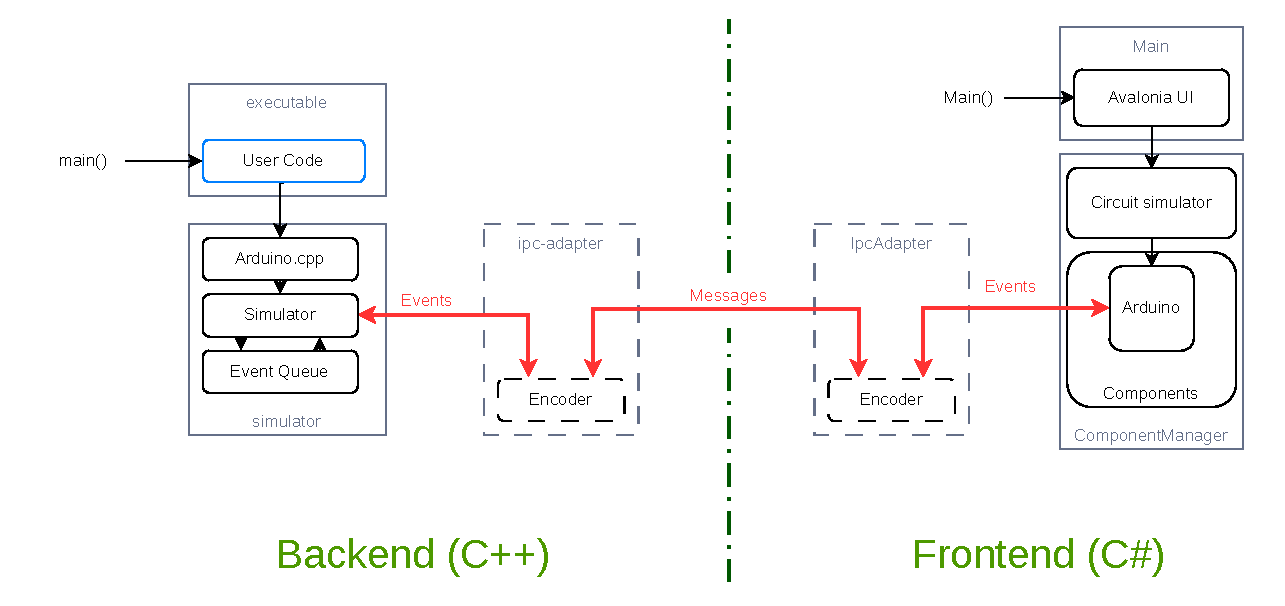
\includegraphics[width=\textwidth, keepaspectratio]{img/overall-architecture.pdf}
    \caption{Top-level architecture overview}
    \label{fig:architecture}
\end{figure}

The Figure \ref{fig:architecture} shows the most important systems in each process. The user code is compiled together with the \texttt{executable} module of the backend. The declarations in the header \texttt{Arduino.h} prepended to the top of the \texttt{.ino} is implemented by a mock library \texttt{Arduino.cpp}. For each observable action an event is created and passed to the singleton \texttt{Simulator} class to compute and put into an event queue. The event is also communicated to the frontend process.

In the frontend the events are consumed by the \texttt{Arduino} component, one of several components predefined as part of the \texttt{ComponentManager} project. This project is responsible for loading user-defined components and scenes, which connect the components together in a circuit. The circuit is simulated in the same project. The user interface is implemented in the \texttt{Main} project using Avalonia UI as a framework. Interacting with the UI may invoke new events in the \texttt{Arduino} component. Those are sent back to the backend's event queue in the same manner as they were received.

The IPC Adapter is an interface implemented in each process responsible for encoding and decoding the events into a standardised format and relaying to the other process.

\section{Inter-process communication}

Implementing processes that depend on each other comes with certain challenges. Processes always run concurrently, so a variety of synchronization techniques must be applied to avoid race conditions. Before that we need to determine how will the processes exchange data. Process is a kernel level mechanism, thus approaches to handle the exchange can vary between operating systems. These mechanisms are what is called \textit{Inter-process communication}, or IPC for short.

\subsection{Considerations}
There is a technical and an engineering reason for splitting the work into more than one process.

The user must be able to have full control over the frontend user interface at all times, even while the Arduino code is being debugged. Every common debugger blocks all running threads of a process, when a breakpoint is hit. \xxx{elaborate} If the GUI has been part of the same process as the systems running the simulation, it would freeze and become unresponsive every time a breakpoint is hit. The only way to avoid this behavior is to separate the GUI to a different process. We want to support breakpoints in our project, as they are the most useful tool in a debugger's toolkit.

Splitting the application into multiple processes is actually a common practice among larger pieces of software. The program of each process can be written in a different programming language and thus delegated into teams with different competencies. They mark clear separation of concerns and force a solid interface design. Each process is easily swappable for another implementation with the same interface while the other processes are still running. In our case, the GUI process could be replaced by a web client, a CLI client, or an IDE add-on.

There are more than a few ways to handle IPC on every OS. The ones that we implemented are \textit{TCP stream} and \textit{shared memory}. These are among the most common approaches available both on Windows and Linux. In either case, we must clearly define what the shared data represent. Although shared memory has more flexibility than TCP, we stuck to sending discrete text or binary messages of predetermined format over time, to keep the implementation simpler and the two approaches interchangable.

Another question is what will we encode in our message. At first we encoded the full state of the simulated Arduino in \textit{snapshots} but due to its various shortcomings we later switched to sending discrete \textit{events}. So the simulator in the backend and its interpratation in the frontend both operate in terms of events, but TCP and shared memory modules only understand the notion of sending and receiving messages with very distinct interfaces. That's why we need to design an adapter in both processes and for both IPC methods that sets up the mechanism and encodes or decodes the passing messages into structured event data the simulation logic understands. The IPC adapter then informs the other systems in it's process any time a new event is received.

\subsection{Snapshotting}

In the early iterations, a snapshot of the Arduino state was sent over one message. That included the pinout state, pin modes, timer, etc. The state was periodically requested by the client with a \textit{Read} message without payload. When a new value is read on an input pin in the frontend, a \textit{Write} message with the state as payload would be sent to the server and the values of input pins would be overwritten atomically to the backend's internal state. 

This approach was easy to implement but flawed. The main issue was the frequency of reads. At lower frequencies, the system is prone to temporal aliasing. \xxx{Find temporal aliasing definition}. Some events, like very short impulses, can be missed completely. This is not much of an issue in purely combinational circuits. But we want our frontend to support stateful components, e.g. shift registers present on the Funshield, which are controlled by digital writes less than a microsecond a part.

Highering the frequency to such an extent is not viable. \xxx{elaborate}

\subsection{Events}\label{subsec:events}

Right now synchronization between processes is maintained by recording every significant event produced by either the backend or the frontend, and sending it to the other process. Each process is equipped with an event queue, that consumes the events in order of the least recent to the most recent. Consuming an event means invoking the appropriate function based on the type of the event with arguments stored in the event's signature. 

The Arduino object in the frontend has no logic on its own, so the only consumed events are those produced by the backend. For that reason a simple queue is sufficient, and no further synchronization is necessary. In the backend however, both simulator's and frontend's events are consumed. Sending an event to the frontend and receiving direct consequeunces of the event back can involve a significant time overhead. In the meantime the simulator produces more events that are consumed almost instantaneously. We need to ensure that the events are consumed in a valid order. We also need a robust queue implementation that isn't prone to race conditions.

An event is labeled with two timestamps. Timestamps don't have to be based on a real clock, the only requirement is that it is a non-decreasing sequence of numbers. The first timestamp sent is the simulation time, the time as perceived by the Arduino being simulated. That is time given by a clock that is started right before the \texttt{setup()} is invoked. It can be manipulated by the user by pausing or slowing down. This is to aid the user while analyzing the logs of the simulator.

The other timestamp included is \textit{Local virtual time} (LVT)\footnotemark. Each process holds its own integer value of LVT. This number is increased with newly produced events and events received from the other process. When a decision has to be made on which event to consume next (like in the case of the backend's queue), the event with lower LVT is chosen. The relation $LVT_{1} > LVT_{2}$ means that the event with $LVT_{1}$ happens after the event with $LVT_{2}$. In other words, event 1 is the consequence of the event 2 regardless of the real time passed between the events.

The rest of the information stored in an event is its type and arguments. The type corresponds to the action taken after the event is consumed, like writing to a pin or changing pin mode. Each type can define up to 3 integer parameters, e.g for a \textit{write} event that is id of the pin, and a digital value we want to write to it. By limiting the number of arguments, we intend to avoid heap allocation of these events, which could considerably slow down the simulation with programs that produce a lot of events in a short time.

There are many ways to encode such an event into a message. Currently the only encoder implemented in this work is the text encoder, which parses values of events into human readable strings separated by a colon. The messages themselves are separated by a semicolon. This particular encoding is quite space ineffective, but it helps a lot during debugging of the IPC systems.

\footnotetext{The terminology and principles are inspired by the \textit{Optimistic synchronization} paradigm in distributed systems. In this paradigm, the events are consumed as fast as possible, and then rolled back once an event with a lower LVT than the ones consumed appears (so called \textit{Time Warp} mechanism). But Time Warp is not viable for simulating code of a high level language like C++ without custom memory management, and in our implementation it isn't even necessary. \cite{fujimoto_parallel_2001}}

\subsection{TCP stream}

Messages can be sent and received through a stream of data on a TCP connection. TCP is commonly used to send data over a network, meaning backend and frontend processes can run on different machines. But listening to a connection on the same machine on the same port works just as well. TCP messages are guaranteed to arrive in the same order as they were sent.

The backend implements the TCP server, while the frontend implements the client. The implementations and design considerations behind these are very different based on the language they were written. But in both cases TCP handlers need to run on their own threads, due to how heavyweight \xxx{elaborate} they are. There is a buffer to which read bytes are stored from an OS network stream. These are passed as a chunk to a higher level message handler that splits the chunk into individual messages according to predetermined delimeter character. When a message needs to be sent from another thread, it is passed to the message handler where it is posted to the end of a queue and is scheduled to be processed by the OS.

There is a minor limitation of IPC over TCP that makes the debugging experience of the user's code uncomfortable. As we established, hitting a breakpoint will block all running threads of the process, including the thread with the TCP handler. When stepping through the lines of the code where events are produced, the TCP thread has to schedule posting of the message with the event, and it takes time for it to be eventually sent. In many cases the TCP thread won't be fast enough to send the message in the time the main thread progresses to the next line where a breakpoint will be hit again. As a result, consequences of the event won't be reflected in the frontend process until another one or more lines have been stepped through. This is the main reason we decided to also implement IPC with memory mapping, even though TCP is fully functional.

\subsection{Shared memory}

Memory mapping is the functionality of an operating system to relate a region of main memory 1:1 to a region in the address space of a process. This is an important idea in establishing a virtual memory of a process, but OS objects can be mapped as well. It could be either a \textit{memory-mapped file}, contents of a disk file moved to the RAM. Or it could be a special OS object called \textit{shared memory}, living in the kernel heap, specifically designed for IPC. In both cases, multiple processes can map the same memory region to their own address space. Thus they have access to the same data.

The terminology and API differ significantly between Linux and Windows, but with the use of the right libraries, the differences can be abstracted away and used as a single concept. So from now on we refer to the idea of mapping the same memory region to multiple address spaces as \textit{shared memory}.

This tool is very powerful, we can address the shared data by pointers as we would with any other data of the process. There is also no need for system calls once the the memory has been mapped. No special instructions need to be used for reading or writing and all changes are immediately visible on all of the processes that map the same region. As long as we do the writes in the simulating thread, we avoid the problem with delayed observations during debugging we encountered with TCP.

In the shared memory region, we establish a data structure that stores messages in a sequential order. We opted for a circular buffer to fully utilize the limited space of the region. There are actually two non-overlapping buffers in the same region together with a few bytes of metadata about their current state. A process consumes messages from one buffer while producing new messages to another. This is to avoid numerous race conditions that would occur while writing and reading from the same buffer while keep the synchronization mechanism lock-free.

As for the metadata, for each buffer a position after the last consumed and produced message is stored. It is important to never store references as pointers in the shared memory itself. The memory region will be most likely mapped to different addresses in each process. Because of that the \textit{producer offset} and \textit{consumer offset} are regular integers denoting the distance from the first adress of the buffer in bytes. When the offsets are equal, it means the buffer is empty. We don't care about concurrent updates of these offsets, one process changes only one of the offsets for the duration of the simulation.

\begin{figure}
    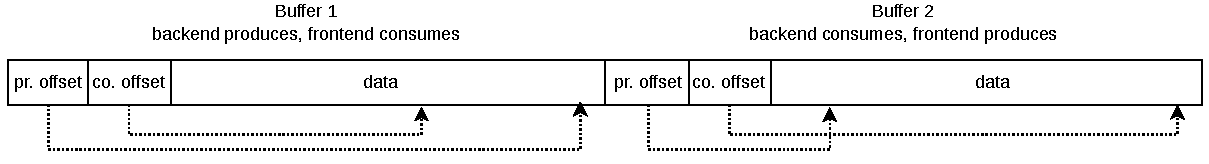
\includegraphics[width=\textwidth, keepaspectratio]{img/circular-buffer.pdf}
    \caption{Memory layout of the shared memory region}
    \label{fig:circular-buffer}
\end{figure}

\section{Backend}

\subsection{The simulation}

\begin{figure}[ht]
    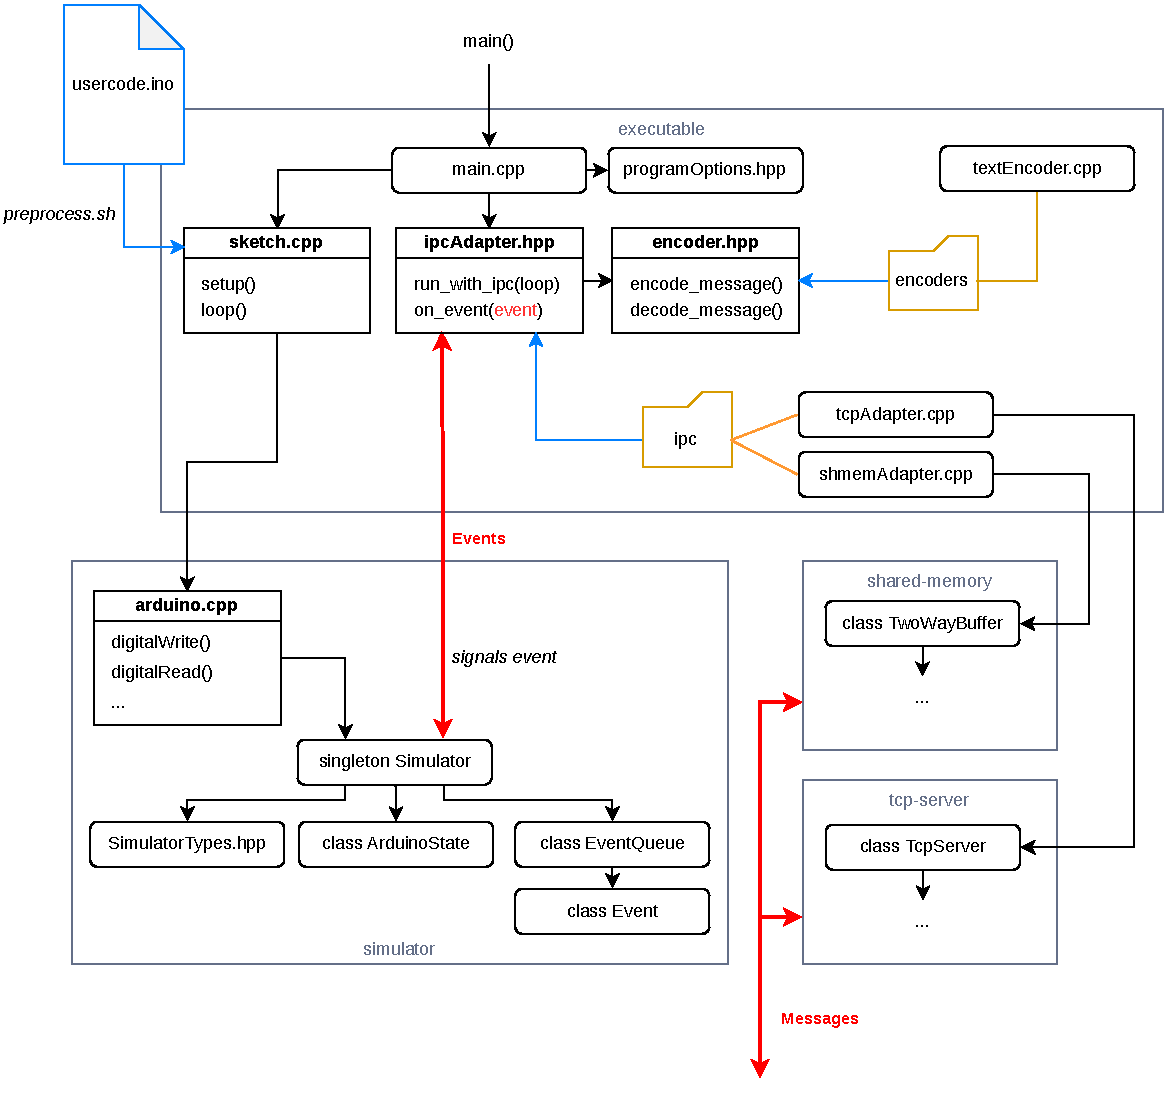
\includegraphics[width=\textwidth, keepaspectratio]{img/backend-architecture.pdf}
    \caption{Backend architecture}
    \label{fig:backend}
\end{figure}

The language choice for backend was obvious, the \texttt{.ino} file is a syntactically valid C++ code. We include the code in the project by passing it as an argument to the \texttt{preprocess.sh} script (\texttt{preprocess.bat} on Windows). Inside we use the \texttt{arduino-cli} tool with the right arguments to apply very light prerpocessing to the file, like adding function declarations to the top or including the \texttt{Arduino.h} header. Important additions are the \texttt{\#line} directives, which link to the definitions in the original \texttt{.ino} file. Thanks to these, breakpoints can be added to the \texttt{.ino} file and debugged as if the file itself was part of the project, completely with stepping through lines and inspection of variables. The file is then saved as \texttt{sketch.cpp} in the directory of the \texttt{executable} module where it is picked up by the CMake configuration and included in the \texttt{main.cpp}. The functions declared by the \texttt{Arduino.h} header file, like \texttt{digitalWrite} or \texttt{millis} are implemented in a custom mock library \texttt{Arduino.cpp} in the \texttt{simulator} module. Instead of instructing the AVR chip, as the real implementation would, the mock definitions create events and pass them to the \texttt{Simulator} for enquing and consumption. 

The \texttt{Simulator} singleton class is the beating heart of the backend. It is responsible for handling the events and the event queue, managing the Arduino state, logging changes and keeping track of time. It is initialized in \texttt{main.cpp} and used frequently throughout the \texttt{executable} and \texttt{simulator} modules. The \texttt{Simulator} holds the instance of the \texttt{ArduinoState} class, representing the digital states on its pins, current pin modes and the inner timer of the Arduino. It also holds the instance of the \texttt{EventQueue}, which stores both local and remote events waiting for consumption. The \texttt{SimulatorTypes.hpp} is a header file with very few type defintions commonly used in the \texttt{simulator} module.

\subsection{Events and IPC}\label{subsec:cpp-events}

The \texttt{Event} struct is just a "recipe" for what changes should the \texttt{Simulator} do to the \texttt{ArduinoState}. It holds a lambda function, corresponging to an event's type that is executed only after the event is put in the event queue and consumed in the order described in the section \ref{subsec:events}. The struct defines static functions that create new event instances with these predefined lambdas with the event type's parameters. When a local event is consumed, i.e. the lambda is executed, the event is signalled back to the \texttt{executable} module through a callback, that has been passed to the \texttt{Simulator} during initialization. This way the event can be sent to an IPC adapter, regardless of the used implementation, without a circular dependency on the \texttt{executable} module.

The IPC adapter itself is an interface of two functions declared in the \texttt{ipcAdapter.hpp}. \texttt{run\_simulator\_with\_ipc} initializes the IPC mechanism. It takes the simulator loop function as an argument and executes it after IPC has been set up. That is because the IPC usually needs to create new threads that cannot be joined before the loop stops running. The loop function itself is defined in \texttt{main.cpp} and it contains both the \texttt{setup()} and \texttt{loop()} calls from the user's code.

The \texttt{on\_event} function of the adapter is the callback passed to the \texttt{Simulator}. It encodes the event into a message and sends over IPC to the remote process. Listening to events of the remote process occurs on a different thread than the one with the simulator loop. Incoming messages are decoded into \texttt{Event} structs and sent directly to the event queue in the \texttt{Simulator}. \texttt{encode\_message} and \texttt{decode\_message} are functions declared in yet another interface in the \texttt{encoder.hpp} header. It's implementations are in the \texttt{encoders} directory, i.e. only \texttt{textEncoder.cpp} at the moment.

Implementations of the IPC adapter are located in the \texttt{ipc} directory. The \texttt{tcpAdapter.cpp} depends on the \texttt{tcp-server} module, while the \texttt{shmemAdatper.cpp} depends on the \texttt{shared-memory} module. Which one is used depends on the chosen compilation target. The \texttt{tcp-server} module contains definition of the TCP server and mechanisms for accepting new connections and handling the stream of data using the \texttt{boost::asio} library. The \texttt{shared-memory} module contains memory mapping mechanisms using the \texttt{boost::interprocess}, implementation of the circular buffer and the producer-consumer pattern using two buffers.

\subsection{Utilities}

\subsubsection{Logger} \label{subsub:logger}

There are additional utility modules not shown in the figure \ref{fig:backend}. One of them is the humble \texttt{logger} used extensively throughout the project. The \texttt{ILogger} abstract class exposes the \texttt{log} function accepting either a raw string or an \texttt{IMessage} abstract struct. Structs inheriting form \texttt{IMessage} represent unified formatting of a message with a timestamp and a level of verbosity. The verbosity levels from the highest to lowest are \textit{Debug}, \textit{Info}, \textit{Warning} and \textit{Error}. The messages of higher verbosity levels can be ommitted from the logs by setting the appropriate command line option. \texttt{ILogger} offers shorthand functions for logging these general messages, but more specific ones can be defined as well.

The module comes with \texttt{FileLogger} implementation of the \texttt{ILogger}. It creates or opens a file and dumps the logs inside. To avoid race conditions while writing to the files, two of these loggers are used in the project. One is owned and used by the \texttt{Simulator} singleton for logging inner workings of the Arduino. The other is owned by the IPC adapter and used for logging the exchanged messages or potential failures of the IPC mechanisms.

\subsubsection{Timer}

The other utility model is \texttt{Timer}. It is used to track time from the start of the simulation. The simulator holds two of these timers, one for \textit{real time} and one for \textit{simulation time}. Although there is no difference between them right now, the intention is to apply effects like stopping or slowing down to the simulation time timer from the frontend, so that functions like \texttt{millis} work consistently with disturbances caused by the frontend. Functions returning real time and simulation time are passed to the file logger as a source of its timestamps.

\section{Frontend}

\subsection{The presentation}

\begin{figure}
    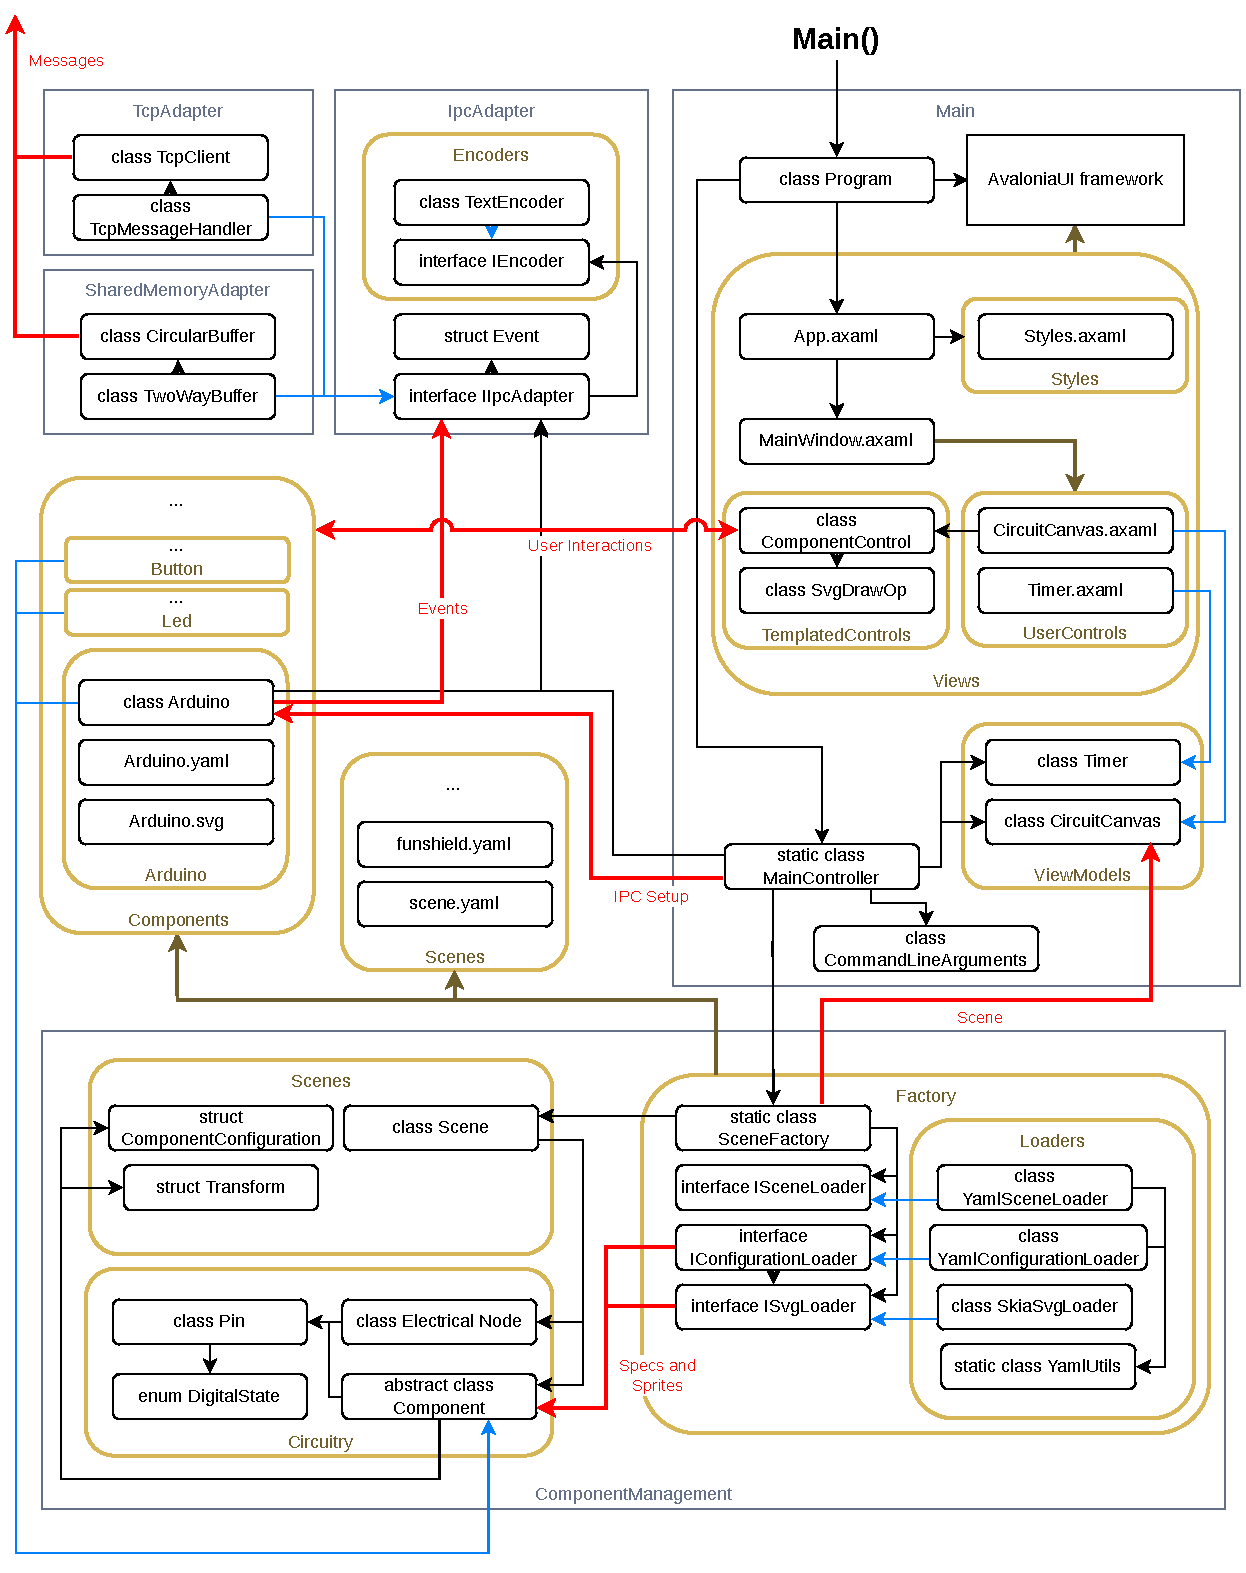
\includegraphics[width=\textwidth, keepaspectratio]{img/frontend-architecture.pdf}
    \caption{Frontend architecture}
    \label{fig:frontend}
\end{figure}

The frontend is written in C\#. We consider the language to be more convenient for writing many of the essential systems than its C++ counterpart. That includes handling the graphics, the user interactions and parsing numerous configuration files needed for extensibility of the application. Libraries are also much easier to set up and compile thanks to NuGet.

For the GUI we decided to use Avalonia UI. Avalonia is a popular open-source cross-platform .NET framework, used by major companies like JetBrains or Unity. It is based on the Microsoft's WPF framework utilising the same XAML markup language and many of the same core principles. We chose it exactly because neither WPF or its cross-platform successor MAUI are available on Linux, one of our target platforms. We only include Avalonia in the Main project of the frontend, as this is the only project responsible for rendering.

Our humble GUI consists mostly of the circuit canvas. A zoomable and pannable space where the \textit{components} of a circuit can be placed to specific coordinates, uncostrained by the usual layout structures of Avalonia. Arrangement of these components is called a \textit{scene}. Each of the component types have its own set of SVG images that are drawn to the canvas. We refer to them as \textit{sprites}. Each individual component always references one of its sprites, conveying the current state to the user. A sprite on the canvas can be clicked on (e.g. a button) to generate some kind of response. Of course, these features are not built into Avalonia, so we need to create custom Avalonia \textit{controls} to achieve them.

\subsubsection{Model-View-ViewModel}

The preferred architecture for Avalonia applications is \textit{MVVM}, or \textit{Model-View-ViewModel}. \textit{View} is the visual layout of the window and its parts. It is written in \textit{XAML} (Extensible Application Markup Language) in files with the \texttt{.axaml} extension. In Avalonia's case, elements of a view are called \textit{controls}. Those can be buttons, labels, containers, etc. 3 types of custom controls can be created in total, our frontend utilizes \textit{user controls} and \textit{custom-drawn controls}. User controls are themselves views built up in XAML from other controls. This is perfect for our \texttt{CircuitCanvas} view, as it is just a list of component controls enveloped in a built-in \texttt{Canvas} panel. The custom-drawn controls are defined as C\# classes, inheriting from the \texttt{Control} class, and defining it's own rendering logic by overriding the \texttt{Render} method \cite{avalonia_custom_controls}.

We need to implement the visuals of our components using custom-drawn controls, as there are no built-in or library controls that can draw a precompiled SVG image and swap it during runtime. Thus we define a \texttt{ComponentControl}, that calls a custom drawing operation in its \texttt{Render} method. That is defined by the \texttt{SvgDrawOp} class, which takes a sprite and a transformation matrix as arguments, applies visual transformations on the image and instructs the Avalonia's rendering pipeline to show it in the parent view.

XAML views bind to data and events in a \textit{viewmodel}, which manipulates with data shown in the view. A model then is the raw data passed to the viewmodel, accessed by some database or a service, or produced by the business logic. View is aware of the viewmodel and viewmodel is aware of the model, but not vice versa. In ideal case, the model should be agnostic about the UI technology used. \cite{avalonia-mvvm}

Our model is the abstract \texttt{Component} class implemented by various types of components, like LEDs, buttons or our Arduino. A list of the \texttt{Component} instances is stored in \texttt{CircuitCanvas} viewmodel, and each instance is passed to a \texttt{ComponentControl} in the \texttt{CircuitCanvas} view. This and all other initialization steps of the application are orchestrated by the static \texttt{MainController} class.

\begin{figure}
    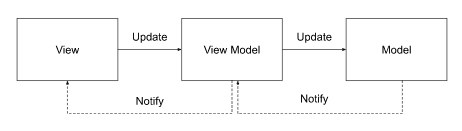
\includegraphics[width=\textwidth, keepaspectratio]{img/mvvm.png}
    \caption{MVVM architecture {\cite{avalonia-mvvm}}}
    \label{fig:mvvm}
\end{figure}

\subsection{The logic}

Only a minor part of the frontend is actually written with Avalonia. The business logic of the aforemention \texttt{Component} model is all encompassed in the \texttt{ComponentManagement} project. That means parsing of the components definition, creating instances of a scene, and the simulation of the circuit. This project is completely unaware, that it will be rendered with Avalonia specifically.

The circuit can be thought of as an unoriented multigraph, where the nodes of the graph are both \textit{electrical nodes} and the \textit{components}. All neighbors of an electrical node are components, and all neighbors of a component are electrical nodes. An edge of the graph represents a conductive connection between an electrical node and a \textit{pin} of a component. Components usually have multiple pins. 

In a digital circuit, an electrical node always obtains one of two digital states, \textit{high} or \textit{low}, which is given by states of pins it is connected to. When a high state is written into a pin, we say it is \textit{driving}. When a low state is written into a pin, it becomes not driving again. The digital state of an electrical node is high precisely when at least one of the pins it is connected to is driving. A change in the state of an electrical node is propagated through all of the connected pins. Components can react to this change by writing new states to their other pins creating a chain reaction of state changes in the circuit.

\subsubsection{Components}

The frontend's user is encouraged to extend the simulation with their own implementations of the abstract \texttt{Component} class. That is done by creating a new \textit{component directory} with the name of the component. The shared path to all component diretories is specified as one of the command line options of the frontend. The static information about the component type is stored as a record \texttt{ComponentConfiguration}, created from the files in the directory. The required files are a YAML file with metadata and at least one SVG file for the sprite. The YAML file contains in the very least a name to identify the component type, and a list of the component's pins. The pins can be defined either as an enumeration of their names, or as a single integer, that represents the total count of unnamed pins identified by their index.

The \texttt{Component} base class provides multiple virtual methods with the \texttt{On*} prefix. These are called upon changes in the circuit or as a result of a user interaction. The most important one is the \texttt{OnPinStateChanged} with the \texttt{Pin} object passed as an argument. This is the primary way of defining the component's logic. \texttt{OnControlPress} and \texttt{OnControlRelease} are other useful methods for interactible components, such as buttons. The base method \texttt{UpdateSprite} changes the rendered sprite to a different one, identified by the name of its SVG file. The base \texttt{GetPin} method returns a \texttt{Pin} object of the component's instance identified either by its name or index. Digital states are read and written through this object. 

Usually, specific pins have inherent semantics of being used only for reading or only for writing. This property can be set explicitly on the \texttt{Pin} object with \texttt{MakeReadOnly} and \texttt{MakeWriteOnly} methods. Read only pins refuse write attempts from the component's logic and write only pins refuse notifying a component with a new state from node's propagation. General pins, defined by method \texttt{MakeGeneral} don't have these constraints. Incorrect use of pins with these semantics is followed by a warning in the simulation logs.

\lstinputlisting[language=yaml, caption={Component configuration example: Led.yaml}]{../frontend/ComponentManagement/Components/Led/Led.yaml}

\subsubsection{Scenes}

The final form of the graph is achieved with creation of the scene. The YAML file of the scene consists of two sections. In the \texttt{Components} section, individual instances of \texttt{Component} subtypes are defined. They must have a unique name, and they should specify a graphic transformation, i.e. position, rotation and scale. This triplet of 2D vectors is composed into a \texttt{Transform} struct and passed into the \texttt{SvgDrawOp} as a transformation matrix. The \texttt{Nodes} section defines individual electrical nodes. A single node in this file is represented as a list of component-pin pairs, where the components are identified by their instance name in the \texttt{Components} section, and the pin is identified by its definition in the \texttt{ComponentConfiguration} of the given \texttt{Component} subtype.

The creation of the scene is comprised of a series of parsers in the \texttt{Factory} directory. There is an interface for each of the file types, i.e. the scene, component configurations and SVG files. Each has exactly one implementation in the \texttt{Loaders} directory, using \texttt{YamlDotNet} and \texttt{SvgSkia} libraries. They are put together in the static \texttt{SceneFactory} class, where component subtypes and instances are finalized. The results is a complete \texttt{Scene} object with initialized \texttt{Component} instances and \texttt{ElectricalNode} lists. The \texttt{SceneFactory} is called by the \texttt{MainController} in the \texttt{Main} project, which passes the scene to the \texttt{CircuitCanvas} viewmodel.

\lstinputlisting[language=yaml, caption={Scene example: minimal.yaml}, label={lst:scene}]{../frontend/Scenes/minimal.yaml}

The example scene in the listing \ref{lst:scene} contains 2 LEDs, 1 button and 1 source of voltage. Source, which has one pin that is always driving, is connected to the 0th pin of the button, which reads a high value of the node. Both LEDs are connected to the 1st pin of the same button. Pressing the button will copy the digital state from pin 0 to pin 1, and thus lights up the LEDs.

\subsection{The Arduino component and IPC}

Arduino is one of the component subtypes of the \texttt{ComponentManagement} project. It is a partial class divided into 2 files. In \texttt{Arduino.cs} it overrides virtual methods and deals with interaction with the circuit. In \texttt{Arduino.Events.cs} it creates events and sends to IPC. It also calls its own method from \texttt{Arduino.cs} when a new event arrives, based on its type and arguments. The adapter is now defined as an \texttt{IIpcAdapter} interface, which is owned by the Arduino component. Events are exchanged through this interface.

The interface is defined in the \texttt{IpcAdapter}, and is implemented by the \texttt{TcpAdapter} and \texttt{SharedMemoryAdapter} projects. It declares methods for connecting to IPC and sending messages. It also declares a C\# event called \texttt{ReceivedEventEvent}, which is invoked after decoding a message incoming from the backend, with the decoded \texttt{Event} struct as an argument. The Arduino component is subscribed to \texttt{ReceivedEventEvent}.

The \texttt{IpcAdapter} project also contains message encoders and a definition of the \texttt{Event} struct. The C++ and the C\# version of the \texttt{Event} struct have the same signature, with the exception of owning a lambda function (described in \ref{subsec:cpp-events}). The lambda is not necessary for the frontend, as there will be only one source of events executed in the frontend, the ones received by the backend. They don't have to be put in a queue, they can be consumed immediately as they come. Frontend also produces events, e.g. when value on an Arduino's input pin is changed from the circuit, but those are never consumed by the frontend. It is the reponsibility of the backend to handle them.

\texttt{IEncoder} and its \texttt{TextEncoder} implementation are analogous to \texttt{encoder.hpp} and \texttt{textEncoder.cpp} in the backend. The interface declares \texttt{EncodeEvent} and \texttt{TryDecodeEvent}, which transcribe events structs into human-readable strings and vice versa.

\subsection{Utilities}

\subsubsection{Logger}

The \texttt{Logger} project is analogous to its backend counterpart (\ref{subsub:logger}). It provides logging to a file with 4 levels of verbosity, that can be set up with a command line argument. Two loggers are used in the frontend as well, one for IPC and one for circuitry logs. There is one additional implemenation of the \texttt{ILogger} called \texttt{CompositeLogger}, which holds list of loggers, and logs into all of them simultaneously. This mechanism anticipates a need for another logger implementation, which will display the log messages in the GUI using Avalonia.
\chapter{Backend implementation} \label{ch:backend}

\section{Simulator module}

\subsection{\texttt{ArduinoState} class}

\begin{lstlisting}[language=csharp, caption={\texttt{ArduinoState} class}]
class $ArduinoState$ {
   public:
    static constexpr uint8_t ANALOG_PIN_COUNT = 6;
    static constexpr uint8_t DIGITAL_PIN_COUNT = 14;
    static constexpr uint8_t PIN_COUNT = 
        ANALOG_PIN_COUNT + DIGITAL_PIN_COUNT;

    using $analog_arr_t$ = $std$::$array$<$analog_t$, ANALOG_PIN_COUNT>;
    using $digital_arr_t$ = $std$::$array$<$digital_t$, DIGITAL_PIN_COUNT>;
    using $pinmode_arr_t$ = $std$::$array$<$PinMode$, PIN_COUNT>;

    void #init_timer#();
    float #get_time#() { return _timer.#deltaTime#(); }

    $analog_arr_t$& #get_analog#() { return _analogPins; }
    double #get_analog#($pin_t$ pin) const;
    bool #set_analog#($pin_t$ pin, $analog_t$ value);

    $digital_arr_t$& #get_digital#() { return _digitalPins; }
    bool #get_digital#($pin_t$ pin) const;
    bool #set_digital#($pin_t$ pin, $digital_t$ value);

    $pinmode_arr_t$& #get_pin_mode#() { return _pinModes; }
    $PinMode$ #get_pin_mode#($pin_t$ pin) const;
    bool #set_pin_mode#($pin_t$ pin, $PinMode$ mode);
   private:
    $Timer$ _timer;
    $analog_arr_t$ _analogPins = {};
    $digital_arr_t$ _digitalPins = {};
    $pinmode_arr_t$ _pinModes = {};
};
\end{lstlisting}

\subsection{\texttt{Simulator} singleton class}

\begin{lstlisting}[language=csharp, caption={\texttt{Simulator} class}]
class $Simulator$ {
   public:
    using $event_callback_fnct$ = 
        $std$::$function$<void(const $Event$&)>;
    using $logger_ptr$ = $std$::$shared_ptr$<logger::$ILogger$>;

    static void #init#(
        $event_callback_fnct$ eventCallback, 
        $logger_ptr$ logger = nullptr);

    static $ArduinoState$& #state#() { return s_instance->_state; }
    static $EventQueue$& #queue#() { return s_instance->_eventQueue; }

    static int64_t #simulation_time#() { return #state#().#get_time#(); }
    static int64_t #real_time#() 
        { return s_instance->_timer.#deltaTime#(); }

    static void #handle_event#($Event$ event);
    static void #handle_events#();

    static void #log_debug#($std$::$string$&& str) 
        { s_instance->_logger->#log_debug#($std$::#move#(str)); }
    static void #log_info#($std$::$string$&& str) 
        { s_instance->_logger->#log_info#($std$::#move#(str)); }
    static void #log_warning#($std$::$string$&& str) 
        { s_instance->_logger->#log_warning#($std$::#move#(str)); }
    static void #log_error#($std$::$string$&& str) 
        { s_instance->_logger->#log_error#($std$::#move#(str)); }
   private:
    static $Simulator$* s_instance;
    $event_callback_fnct$ f_eventCallback;
    $logger_ptr$ _logger;
    $ArduinoState$ _state;
    $EventQueue$ _eventQueue;
    $Timer$ _timer;
};
\end{lstlisting}

\subsection{\texttt{Event} struct}

\begin{lstlisting}[language=csharp, caption={\texttt{Event} struct}]
struct $Event$ {
   public:
    enum class $Type$ { Write, PinMode, Reboot };

    $Type$ type;
    int64_t timestampMicros;
    int64_t localVirtualTime;
    $std$::$function$<void()> action;

    static constexpr int MAX_ARGS = 3;
    $std$::$array$<int, MAX_ARGS> args;

    template <typename... Args>
    $Event$($Type$ type, Args... arguments);
    $Event$() {}

    size_t #id#() const { return _id; }
    $std$::$string$ #to_string#();

    static $Event$ #write#($pin_t$ pin, $digital_t$ value);
    static $Event$ #set_pinmode#($pin_t$ pin, $PinMode$ mode);
    static $Event$ #reboot#();
   private:
    static size_t s_nextEventId;
    size_t _id;
};
\end{lstlisting}

\subsection{\texttt{EventQueue} class}

\begin{lstlisting}[language=csharp, caption={\texttt{EventQueue} class}]
class $EventQueue$ {
   public:
    void #enqueue_local#($Event$& event);
    void #enqueue_remote#($Event$ event);
    void #execute_next_event#();

    $Event$& #last_executed_event#() 
        { return _processedEvents.#back#(); }
    bool #is_empty#() const 
        { return _localEvents.#empty#() && _remoteEvents.#empty#(); }
    int64_t #next_lvt#() const { return _nextLvt; }
    int64_t #last_lvt#() const { return _lastLvt; }

   private:
    $std$::$queue$<$Event$> _localEvents;
    $std$::$queue$<$Event$> _remoteEvents;
    $std$::$queue$<$Event$> _processedEvents;
    int64_t _nextLvt;
    int64_t _lastLvt;
    int64_t _maxGvtFallback;

    void #clear#();
    size_t #earliest_queue_lvt#(const $std$::$queue$<$Event$>& queue);
};
\end{lstlisting}

\subsection{\texttt{Arduino.cpp}}

\section{Executable module}

\subsection{\texttt{main.cpp}}

\begin{lstlisting}[language=csharp, caption={\texttt{main.cpp}}]
using $logger_t$ = logger::$FileLogger$;
using namespace $arguino$::$simulator$;
$ProgramOptions$ options;

void #init_simulator#(
    $Simulator$::$event_callback_fnct$ eventCallback)
{
    auto logPath = $std$::$filesystem$::#absolute#(
        options.SimulatorLogPath);
    auto logger = $std$::#make_shared#<$logger_t$>(logPath);

    $Simulator$::#init#(eventCallback, logger);
    logger->timerFunction = $Simulator$::#simulation_time#;
    logger->verbosityLevel = options.Verbosity;
}

void #simulator_loop#()
{
    $Simulator$::#state#().#init_timer#();

    $Simulator$::#handle_event#($Event$::#reboot#());
    $Simulator$::#log_info#("Simulator initialized.");
    #setup#();
    $Simulator$::#log_info#(
        "setup() finished successfully. Running loop().");

    while (true) {
        #loop#();
    }
}

int #main#(int argc, char** argv)
{
    options = #parse_arguments#(argc, argv);
    #init_simulator#(on_event);
    #run_simulator_with_ipc#(#simulator_loop#, options);
}
\end{lstlisting}

\subsection{\texttt{ipcAdapter.hpp}}

\begin{lstlisting}[language=csharp, caption={\texttt{ipc\_adapter.hpp}}]
using $logger_t$ = logger::$FileLogger$;
using $loop_fnct$ = $std$::$function$<void()>;
using $init_fnct$ = $std$::$function$<void(
    arguino::simulator::$Simulator$::$event_callback_fnct$)>;

static $std$::$shared_ptr$<$logger_t$> IpcLogger;

void #run_simulator_with_ipc#(
    $loop_fnct$ loopFunction, 
    const $ProgramOptions$& options);

void #on_event#(const arguino::simulator::$Event$& event);

inline void #init_ipc_logger#(const $ProgramOptions$& options)
{
    auto loggerAbsolutePath = $std$::$filesystem$::#absolute#(
        options.IcpLogPath);
    IpcLogger = $std$::#make_shared#<$logger_t$>(loggerAbsolutePath);

    IpcLogger->verbosityLevel = options.Verbosity;
    IpcLogger->timerFunction = 
        arguino::simulator::$Simulator$::#real_time#;
}
\end{lstlisting}

\subsection{\texttt{tcpAdapter.cpp}}

\begin{lstlisting}[language=csharp, caption={\texttt{tcp\_adapter.cpp}}]
using namespace arguino::simulator;
using $tcp_server_t$ = arguino::tcp::$TcpServer$;
static $std$::$unique_ptr$<$tcp_server_t$> _tcpServer;

void #on_event#(const $Event$& event)
{
    auto message = #encode_event#(event);
    if (message == UNKNOWN_EVENT) {
        IpcLogger->#log_error#(
            "Encountered unknown event type; skipping.");
        return;
    }

    IpcLogger->#log_debug#("Enqueuing message " + message);
    _tcpServer->#post_message#(message);
}

static void #on_received_tcp_message#(const $std$::$string$ message)
{
    $Event$ event;
    if (#decode_event#(message, event)) {
        $Simulator$::#queue#().#enqueue_remote#(event);
    }
    else {
        IpcLogger->#log_error#(
            "Could not decode event from message " + message);
    }
}

static void #run_tcp#() { _tcpServer->#launch#(); }

void #run_simulator_with_ipc#(
    $loop_fnct$ loopFunction, 
    const $ProgramOptions$& options)
{
    #init_ipc_logger#(options);
    _tcpServer = $std$::#make_unique#<$tcp_server_t$>(
        options.TcpPort, on_received_tcp_message, IpcLogger);

    $std$::$thread$ tcp_thread(#run_tcp#);
    IpcLogger->#log_info#("Tcp Server launched");
    loopFunction();
    tcp_thread.#join#();
}
\end{lstlisting}

\subsection{\texttt{shmemAdapter.cpp}}

\begin{lstlisting}[language=csharp, caption={\texttt{shmem\_adapter.cpp}}]
using namespace arguino::shmem;
using namespace arguino::simulator;

constexpr uint8_t MESSAGE_DELIMETER = ';';
static $TwoWayBuffer$* _shmem;

void #on_event#(const $Event$& event)
{
    auto message = #encode_event#(event);
    if (message == UNKNOWN_EVENT) {
        IpcLogger->#log_error#(
            "Encountered unknown event type while encoding.");
        return;
    }

    if (!_shmem->#write#(message + ';')) {
        IpcLogger->#log_error#(
            "Could not write to shared memory buffer, "
            "not enough available space.");
    }
    else {
        IpcLogger->#log_debug#(
            "Written message to producer buffer: " + message);
    }
}

static void #run_shmem_consumer#()
{
    while (true) {
        while (!_shmem->#consumer#().#is_empty#()) {
            $std$::$vector$<uint8_t> data = 
                _shmem->#consumer#().#consume_until#(
                    MESSAGE_DELIMETER);
            if (data.#empty#()) {
                IpcLogger->#log_error#(
                    "A span of incoming message could not "
                    "be determined, skipping.");
                continue;
            }

            $std$::$string$ message(data.#begin#(), data.#end#());
            IpcLogger->#log_debug#(
                "Read message from consumer buffer: " + message);

            $Event$ event;
            if (#decode_event#(message, event)) {
                $Simulator$::#queue#().#enqueue_remote#(event);
            }
            else {
                IpcLogger->#log_error#(
                    "Could not decode event from message " + message);
            }
        }
    }
}

void #run_simulator_with_ipc#(
    $loop_fnct$ loopFunction, 
    const $ProgramOptions$& options)
{
    #init_ipc_logger#(options);
    _shmem = new $TwoWayBuffer$(
        options.ShmemName, options.ShmemSizePages);

    $std$::$thread$ consumer_thread(#run_shmem_consumer#);
    IpcLogger->#log_info#("Shared memory buffer intitialized.");

    loopFunction();
    consumer_thread.#join#();
}
\end{lstlisting}

\subsection{\texttt{textEncoder.cpp}}

\begin{lstlisting}[language=csharp, caption={\texttt{encoder.cpp}}]
using namespace arguino::simulator;

constexpr char PART_DELIMETER = ':';
constexpr char COMMON_PART_FORMAT[] = "{:012}:{:07}:";
constexpr char WRITE_FORMAT[] = "W:{:02}:{}";
constexpr char PINMODE_FORMAT[] = "P:{:02}:{}";
constexpr char REBOOT_FORMAT[] = "R";

constexpr int COMMON_PARTS = 3;
constexpr int MAX_ARGS = 3;
constexpr int MAX_PARTS = 6;

using $parts_array_t$ = $std$::$array$<$std$::$string_view$, MAX_PARTS>;

static $std$::$string$ #encode_write#(const $Event$& e)
    { return $std$::#format#(WRITE_FORMAT, e.args[0], e.args[1]); }

static $std$::$string$ #encode_pinmode#(const $Event$& e)
    { return $std$::#format#(PINMODE_FORMAT, e.args[0], e.args[1]); }

static $std$::$string$ #encode_reboot#(const $Event$& e)
    { return REBOOT_FORMAT; }

$std$::$string$ #encode_event#(const $Event$& event)
{
    $std$::$string$ commonPart = $std$::#format#(
        COMMON_PART_FORMAT, 
        event.timestampMicros, 
        event.localVirtualTime);

    switch (event.type) {
        case $Event$::$Type$::Write:
            return commonPart + #encode_write#(event);
        case $Event$::$Type$::PinMode:
            return commonPart + #encode_pinmode#(event);
        case $Event$::$Type$::Reboot:
            return commonPart + #encode_reboot#(event);
        default:
            return UNKNOWN_EVENT;
    }
}

bool #decode_int#($std$::$string_view$ str, int64_t& out) { ... }
bool #decode_int#($std$::$string_view$ str, int& out) { ... }
$parts_array_t$ #split#($std$::$string_view$ messageView) { ... }

bool #decode_event#(const $std$::$string$& message, $Event$& event)
{
    $parts_array_t$ parts = #split#(message);
    $std$::$array$<int, MAX_ARGS> args;

    for (int i = 0; i < MAX_ARGS; ++i) {
        if (!#decode_int#(parts[COMMON_PARTS + i], args[i])) break;
    }

    if (parts[2] == "W") {
        event = $Event$::#write#(args[0], args[1]);
    }
    else if (parts[2] == "P") {
        event = $Event$::#set_pinmode#(args[0], ($PinMode$)args[1]);
    }
    else {
        return false;
    }
    if (!#decode_int#(parts[0], event.timestampMicros) || 
        !#decode_int#(parts[1], event.localVirtualTime)) {
        return false;
    }
    return true;
}
\end{lstlisting}

\section{TCP Server module}

\subsection{\texttt{TcpServer} class}

\begin{lstlisting}[language=csharp, caption={\texttt{TcpServer} class}]
class $TcpServer$ {
   public:
    using $handler_t$ = $ConnectionHandler$;
    using $logger_ptr$ = $std$::$shared_ptr$<logger::$ILogger$>;

    $TcpServer$(
        uint16_t port, 
        $handler_t$::$message_funct$ messageHandler, 
        $logger_ptr$ logger);

    void #launch#();
    void #post_message#(const $std$::$string$& message);
    bool #is_connected#() const;

   private:
    $boost$::$asio$::$io_context$ _ioContext;
    $boost$::$asio$::$ip$::$tcp$::$endpoint$ _endpoint;
    $boost$::$asio$::$ip$::$tcp$::$acceptor$ _acceptor;
    uint16_t _port;

    $std$::$shared_ptr$<$handler_t$> _connectionHandler;
    $std$::$mutex$ _connectionMutex;
    $std$::$condition_variable$ _connectionCv;
    $handler_t$::$message_funct$ _messageHandler;
    $logger_ptr$ _logger;

    void #start_accepting#();
};
\end{lstlisting}

\subsection{\texttt{ConnectionHandler} class}

\begin{lstlisting}[language=csharp, caption={\texttt{ConnectionHandler} class}]
class $ConnectionHandler$ : 
    public $std$::$enable_shared_from_this$<$ConnectionHandler$> {
   public:
    static constexpr char MESSAGE_DELIMITER = ';';
    static constexpr size_t MAX_QUEUE_SIZE = 100;
    using $self_ptr$ = $std$::$shared_ptr$<$ConnectionHandler$>;
    using $logger_ptr$ = $std$::$shared_ptr$<logger::$ILogger$>;
    using $message_funct$ = $std$::$function$<void(const $std$::$string$&)>;

    $ConnectionHandler$(
        $boost$::$asio$::$io_context$& ioContext, 
        $message_funct$ messageHandler, 
        $logger_ptr$ logger);
    static $self_ptr$ #create#(
        $boost$::$asio$::$io_context$& ioContext, 
        $message_funct$ messageHandler, 
        $logger_ptr$ logger);

    void #handle#();
    void #post_message#(const $std$::$string$& message);
    $boost$::$asio$::$ip$::$tcp$::$socket$& #socket#() 
        { return _socket; }
    bool #is_connected#() const { return _isConnected; }

   private:
    $boost$::$asio$::$io_context$::$executor_type$ _executor;
    $boost$::$asio$::$ip$::$tcp$::$socket$ _socket;
    $std$::$string$ _incomingBuffer;
    $std$::$queue$<$std$::$string$> _outboxQueue;
    $std$::$mutex$ _queueMutex;
    $std$::$condition_variable$ _queueCv;
    size_t _connectionId;
    static size_t _nextConnectionId;
    bool _isConnected;
    $std$::$atomic$<bool> _isWriting;
    $message_funct$ _messageHandler;
    $logger_ptr$ _logger;

    void #handle_message#(
        $boost$::$system$::$error_code$ error, 
        size_t messageSize);
    void #write_from_queue#();
    void #disconnect#();
};
\end{lstlisting}

\section{Shared Memory module}

\subsection{\texttt{MemoryRegion} class}

\begin{lstlisting}[language=csharp, caption={\texttt{MemoryRegion} class}]
class $MemoryRegion$ {
   public:
    using $shmem_t$ = 
        $boost$::$interprocess$::$shared_memory_object$;
    using $shmem_region_t$ = 
        $boost$::$interprocess$::$mapped_region$;

    $MemoryRegion$(
        const $shmem_t$& shmemObject, 
        size_t offset, 
        size_t size);

    size_t #size#() { return _mappedRegion.#get_size#(); }
    uint8_t* #begin#() 
        { return (uint8_t*)_mappedRegion.#get_address#(); }
    uint8_t* #end#() { return #begin#() + #size#(); }

    template <typename T>
    T& #at#(size_t offset);
    uint8_t* #at#(size_t offset) { return #begin#() + offset; }
    size_t #offset#(void* ptr) 
        { return (uint8_t*)ptr - #begin#(); }

   private:
    $shmem_region_t$ _mappedRegion;
};
\end{lstlisting}

\subsection{\texttt{CircularBuffer} class}

\begin{lstlisting}[language=csharp, caption={\texttt{CircularBuffer} class}]
class $CircularBuffer$ {
   public:
    struct $iterator_t$;
    friend struct $iterator_t$;

    using $shmem_t$ = 
        $boost$::$interprocess$::$shared_memory_object$;

    static constexpr size_t PRODUCER_PTR_LOCATION = 0;
    static constexpr size_t CONSUMER_PTR_LOCATION = 8;
    static constexpr size_t BUFFER_LOCATION = 16;
    $CircularBuffer$() = default;
    $CircularBuffer$(
        const $shmem_t$& shmemObject, 
        size_t offset, 
        size_t size);

    bool #is_empty#();
    size_t #buffer_size#() 
        { return _memoryRegion->#size#() - BUFFER_LOCATION; }
    size_t #bytes_filled#();
    size_t #bytes_available#() 
        { return #buffer_size#() - #bytes_filled#(); }

    template <typename T>
        requires $std$::$is_trivially_copyable_v$<T>
              && (!$std$::$ranges$::$contiguous_range$<T>)
    bool #write#(const T& data);

    template <$std$::$ranges$::$contiguous_range$ TRange>
    bool #write#(const TRange& data);

    $std$::$vector$<uint8_t> #consume_until#(uint8_t delimeter);

   private:
    $std$::$unique_ptr$<$MemoryRegion$> _memoryRegion;

    $iterator_t$ #begin#();
    $iterator_t$ #end#();
    $iterator_t$ #at#(size_t offset);
    $iterator_t$ #producer_it#();
    $iterator_t$ #consumer_it#();
    void #write_producer#($iterator_t$ producer_it);
    void #write_consumer#($iterator_t$ consumer_it);
};
\end{lstlisting}

\subsection{\texttt{TwoWayBuffer} class}

\begin{lstlisting}[language=csharp, caption={\texttt{TwoWayBuffer} class}]
class $TwoWayBuffer$ {
   public:
    using $shmem_t$ = 
        $boost$::$interprocess$::$shared_memory_object$;

    $TwoWayBuffer$(const $std$::$string$& shmemName, size_t sizeInPages);
    ~$TwoWayBuffer$();

    template <typename T>
    bool #write#(const T& data);

    $std$::$vector$<uint8_t> #consume_until#(uint8_t delimeter);
    $CircularBuffer$& #producer#() { return _producer; }
    $CircularBuffer$& #consumer#() { return _consumer; }
    $std$::$string$& #name#() { return _name; }
    size_t #pages#() { return _pages; }
    size_t #size#();

   private:
    $std$::$string$ _name;
    size_t _pages;
    $shmem_t$ _shmemObject;
    $CircularBuffer$ _producer;
    $CircularBuffer$ _consumer;
};
\end{lstlisting}
\chapter{Frontend implementation} \label{ch:frontend}

\section{Component Management project}

\section{Main project with Avalonia UI}

\section{IPC Adapter project}

\section{TCP Adapter project}

\section{Shared Memory Adapter project}

\section{Logger project}
\chapter{User documentation} \label{ch:docs}

\section{Compiling and running the simulator with Arduino code}

\subsection{Build process and usage examples}

First make sure you comply with the software prerequisites from the section \ref{prerequisits}. Make sure your Boost libraries can be found by the CMake metabuild system from your development environment. For further information, please follow the Boost's getting started guide \cite{boost_get_started}. After that, we can preprocess the sketch, compile it with the simulator, and run the simulator together with the frontend.

\subsubsection{Backend process}
\begin{enumerate}
    \item Run \texttt{preprocess.sh} with the sketch directory. On Windows, use the \texttt{preprocess.bat} script instead. For example:
    
    \begin{lstlisting}[language=shell]
    ./preprocess.sh tests/buttons.
    \end{lstlisting}
    
    \item Build \texttt{backend/CMakeLists.txt}. Available targets are:
    
    \begin{description}
        \item[\texttt{arguino-shared-memory}] for IPC over shared memory
        \item[\texttt{arguino-tcp}] for IPC over TCP connection
        \item[\texttt{arguino}] is an alias for the shared memory version (Default and preferred version).
    \end{description}

    \item Run \footnotemark
    \begin{lstlisting}[language=shell]
    <build dir>/executable/<build target>
    \end{lstlisting}
    
\end{enumerate}

\footnotetext{On Windows, the \texttt{.exe} extension is usually appended, i.e. \texttt{.../<build target>.exe}.}

\subsubsection{Frontend process}
\begin{enumerate}
    \item Build \texttt{frontend/gui.sln}.
    \item Run the \texttt{Gui} executable\footnotemark with the desired scene. For example, in the \texttt{frontend} directory call:
    
    \begin{lstlisting}[language=shell]
    <build dir>/Gui -s ./Scenes/buttons.yaml. 
    \end{lstlisting}
    
    If you built the TCP version of the backend, be sure to add the flag \texttt{-i Tcp}.
    
\end{enumerate}

For frontend and backend to communicate properly, it is necessary that they connect to the same IPC object. For TCP it is the port (\texttt{-p} option for both programs), and for shared memory it is the shared memory's object name (\texttt{-{}-shmem-name} option for both programs). These default to the same value for both of the aforementioned options, port \texttt{8888} and memory named \texttt{Arguino-ipc}.

\footnotetext{\texttt{Gui.exe} on Windows}

\subsection{Command-Line Arguments}
Listed below are all the available command line options for the backend and frontend executables. Default values, if defined, are specified in the square brackets. Expected arguments are in the angle brackets. For arguments accepting only specific enumeration of values, all available values are listed in the angle brackets seperated by a vertical bar (\texttt{|}). In square brackets is the default value used, when the option is omitted.


\subsubsection{Backend}
\begin{description}
    \item[\texttt{-{}-log-simulator <path>}] Path to the log file for simulator events. [\texttt{./core.log}]
    \item[\texttt{-{}-log-ipc <path>}] Path to the log file for Inter-Process Communication (IPC). [\texttt{./core\_ipc.log}]
    \item[\texttt{-v, -{}-verbosity <Debug | Info | Warning | Error>}] Verbosity level of the log files. [\texttt{Info}]
\end{description}

\subsubsection{Frontend}
\begin{description}
    \item[\texttt{-s, -{}-scene <path>}] Path to the \texttt{.yaml} scene definition file. [\texttt{./scene.yaml}]
    \item[\texttt{-c, -{}-components <path>}] Path to the directory containing component definitions. [\texttt{./ComponentManager/Components}]
    \item[\texttt{-i, -{}-ipc <None | Tcp | Shmem>}] Inter-process communication technology utilized for connecting with the simulator. [\texttt{Shmem}]
    \item[\texttt{-{}-log-circuit <path>}] Path to the log file for general circuitry events. [\texttt{./frontend.log}]
    \item[\texttt{-{}-log-ipc <path>}] Path to the log file for IPC events. [\texttt{./frontend\_ipc.log}]
    \item[\texttt{-v, -{}-verbosity <Debug | Info | Warning | Error>}] Verbosity level of the log files. [\texttt{Info}]
\end{description}

\subsubsection{Common for TCP usage}
\begin{description}
    \item[\texttt{-p, -{}-port <int>}] TCP port to listen to. [\texttt{8888}]
\end{description}

\subsubsection{Common for shared memory usage}
\begin{description}
    \item[\texttt{-{}-shmem-name <string>}] Name of the memory-mapped file. [\texttt{Arguino-ipc}]
    \item[\texttt{-{}-shmem-size <int>}] Size of the memory-mapped region per circular buffer, specified in pages (usually $page = 4096B$). [\texttt{1}]
\end{description}

\section{Defining components and scenes} \label{sec:component_spec}
Extensibility of the frontend through custom components and circuits is an important part the project. Here are necessary steps and requirements to create and use new components.

\subsection{Required file structure}
All of the components must reside in one directory, referred to as \textit{definitions directory}. Each component is represented by exactly one directory, referred to as \textit{component directory}, placed in the definitions directory. The definitions directory must be supplied through the \texttt{-c} command line argument. These files must be present in the component directory:

\begin{itemize}
    \item C\# behavior script
    \item YAML component configuration
    \item One or more .svg images
\end{itemize}

The yaml file must have the same name as the component directory, i.e. \texttt{MyComponent/MyComponent.yaml}. The SVGs will be referenced in behavior script by their file name, excluding the .svg extension. For example \texttt{image.svg} will be referred to as \texttt{image}.

\subsubsection{Notes on used YAML notation} \label{yaml_notation}
In the next subsections, we will describe the expected structures of the YAML files using this notation:
\begin{itemize}
  \item angle brackets must be replaced by proper parameters, i.e. \texttt{name: <string>}
  \item properties with question mark are optional, i.e. \texttt{optional?: ...}
  \item Vector2 is represented as a string of 2 float values separated by a space, i.e. \texttt{vector: 7.27 6.9} 
\end{itemize}

\subsection{Component configuration file specification} \label{subsec:component_spec}
This file defines common properties of the custom component type.

\begin{lstlisting}[language=yaml, caption={YAML configuration file structure}]
name: <string>
description?: <string>
imageSize?: <Vector2>
pins?: <uint>
pinNames?:
    - <string>
    - ...
    - ...
\end{lstlisting}

\begin{description}
    \item[\texttt{name}] Name of the component type as displayed in the UI. (not used yet)
    \item[\texttt{description}] Brief description of the component as displayed in the UI. (not used yet)
    \item[\texttt{imageSize}] Desired size of the component's sprites in pixels for default zoom level of the canvas. Defaults to <50, 50>.
    \item[\texttt{pins}] Number of unnamed pins. These pins are identified by their 0-based index in both the scene definition and in the component logic.
    \item[\texttt{pinNames}] List of unique names for each pin. These pins are identified by their given name in both the scene defintion and in the component logic.
\end{description}

\lstinputlisting[language=yaml, caption={Component configuration example: Led.yaml}]{../frontend/ComponentManagement/Components/Led/Led.yaml}

\subsection{Component behavior script specification}
How does the component interact with the rest of the circuit is described by the C\# class with the named the same as the component type. This class must inherit from the abstract \texttt{Component} class. The file containg the class must be added to the \texttt{ComponentManagement.csproj} project. In order to compile, the user's class must also define a constructor like this:

\begin{lstlisting}[language=csharp]
    public #MyComponent#(string definitionPath) 
    : base(definitionPath) { ... }
\end{lstlisting}

However, no code is required in the body of the constructor. The constructor can be used for initialization of properties known before the scene is created. The \texttt{Component} class provides most of the necessary API.

\subsubsection{Component functions and properties}
\begin{description}
    \item[\texttt{virtual void OnInitialized()}]
    Gets called when all of the component instances have been initialized and scene created.

    \item[\texttt{virtual void OnPinConnected(Pin)}]
    Gets called when a component's pin connects to an electric node. The connected pin is passed as argument.

    \item[\texttt{virtual void OnPinDisconnected(Pin)}]
    Gets called when a component's pin disonnects from an electric node. The disconnected pin is passed as argument.

    \item[\texttt{virtual void OnPinStateChanged(Pin)}]
    Gets called when a component's pin detected a change in digital state of a node it has been connected to. It can be thought of as changing input value on the pin. Pins set to WriteOnly mode by design don't detect this change. The detected pin is passed as argument.

    \item[\texttt{virtual void OnControlPress(Vector2)}]
    Gets called when the component has been pressed on the circuit canvas. The cursor position at the time of the press is passed as argument.

    \item[\texttt{virtual void OnControlRelease}]
    Gets called when the component has been released on the circuit canvas.

    \item[\texttt{void UpdateSprite(string)}]
    Changes the .svg image drawn to the canvas. The new image is given by the svg name specified in the argument.

    \item[\texttt{Pin? GetPin(string)}]
    Returns a Pin object with the name given in the argument. The name must be defined in the component's \texttt{namedPins} list. Returns null if no such pin exists.

    \item[\texttt{Pin? GetPin(uint)}]
    Returns a Pin object with the id given in the argument. The allowed range of Ids is from \texttt{0} to $pins + namedPins.Length$. With unnamed pins starting from the id \texttt{0} and named pins starting from the id \texttt{pins}. Returns null if the pin id is out of range.
\end{description}

\subsubsection{Pin functions and properties}
\begin{description}
    \item[\texttt{uint Pin.Id}]
    Id of the pin, as described in the \texttt{GetPin(uint)} section.

    \item[\texttt{string Pin.Name}]
    Name of the pin as described in the component configuration.

    \item[\texttt{bool Pin.IsDriving}]
    True if the pin is driving. That is, if it actively forces the digital state on the connected node to be high. If the node has at least 1 driving pin, it's digital state will be high. It will be low otherwise.

    \item[\texttt{bool Pin.IsHigh}]
    True if the digital state of the connected node is high.

    \item[\texttt{bool Pin.IsLow}]
    True if the digital state of the connected node is low.

    \item[\texttt{bool Pin.IsWriteOnly}]
    Write only pins don't react to changes in the connected node's digital state.

    \item[\texttt{bool Pin.IsReadOnly}]
    Read only pins cannot be set to driving.

    \item[\texttt{bool Pin.IsConnected}]
    Whether is the pin connected to any electrical node.

    \item[\texttt{void Pin.MakeReadOnly()}]
    Sets the pin to read only mode. Read only pins cannot be set to driving.

    \item[\texttt{void Pin.MakeWriteOnly()}]
    Sets the pin to write only mode. Write only pins don't react to changes in the connected node's digital state.

    \item[\texttt{void Pin.MakeGeneral()}]
    Sets the pin to general mode. General pins don't pose any restrictions to reading or writing.

    \item[\texttt{void Pin.SetValue(bool)}]
    If the argument is true, it sets the pin to be driving. Otherwise, the pin set to not drive.

    \item[\texttt{void Pin.SetHigh()}]
    Sets the pin to be driving. Same as \texttt{SetValue(true)}.

    \item[\texttt{void Pin.SetLow()}]
    Sets the pin to be not driving. Same as \texttt{SetValue(false)}.
\end{description}

\subsection{Defining scenes} \label{subsec:scene_spec}
The scene YAML file describes component instances present in the scene, and how are their pins connected together in nodes. The path of this file is supplied through the \texttt{-s} command line argument. There are no restriction to where the scene file has to be placed.

\begin{lstlisting}[language=yaml, caption={YAML scene file structure}]
components:
  <Type name>:
    <Instance name>:
      position: <Vector2>
      rotation?: <float>
      scale?: <Vector2>
    <Instance name>:
      ...
nodes:
  - [ <Instance name>.<Pin name>, ...]
  - ...
  - ...
\end{lstlisting}

\begin{description}
    \item[\texttt{components}]
    Dictionary of component type objects. These objects are dictionaries of component instances of that type. These instances define properties of the individual components. 

    \item[\texttt{Type name}]
    String. Name of the component type. This must match the component directory name.

    \item[\texttt{Instance name}]
    String. Name of the component instance. It identifies the instance within the node definition and in the UI. It must be unique across all instances within the components dictionary.

    \item[\texttt{position}]
    Coordinates on the circuit canvas, with origin in the upper left corner.

    \item[\texttt{rotation}]
    Clockwise rotation angle in degrees on the circuit canvas.

    \item[\texttt{scale}]
    Relative scaling along x an y axis on the circuit canvas.

    \item[\texttt{nodes}]
    List of lists. The inner list represents all pins connected to the same electrical node. Its element is an instance-pin pair separated by a dot. Instance name must be present in the components dictionary. Pin name must be present in the component's configuration. In the case of unnamed pins, pin name is simply its index.
\end{description}

\lstinputlisting[language=yaml, caption={Scene example: minimal.yaml}, label={lst:scene}]{../frontend/Scenes/minimal.yaml}

The example scene in the listing \ref{lst:scene} contains 2 LEDs, 1 button and 1 source of voltage. Source, which has one pin that is always driving, is connected to the 0th pin of the button, which reads a high value of the node. Both LEDs are connected to the 1st pin of the same button. Pressing the button will copy the digital state from pin 0 to pin 1, pin 1 becomes driving, and thus lights up the LEDs.

\section{IPC interface}
This section describes how to set up IPC communication of a custom frontend application with the backend simulator. The two processes can communicate together either via TCP connection or through shared memory. The only requirement for a TCP connection, is that the client on the frontend listens to the same port as the server on the backend. IPC over shared memory requires a few more considerations, so that the memory accesses match the memory layout of shared internal structure created by the backend. This structure is described in the subsection \ref{shmem_specs};

The processes communicate using concrete events with up to 3 integer arguments. These events are encoded into a human readable text messages, seperated by a common delimeter. The messages are then sent over IPC.

\subsection{Text message format}
Individual messages are delimited by the semicolon character (\texttt{;}). The individual values within one message are delimited by the colon character (\texttt{:}). The integer values are written in decimal system, using the ASCII characters of the actual digits. The semantics of these values are better described in the chapter about architecture, subsection \ref{subsec:events}. The format of the message then looks as the following:

\begin{lstlisting}[
    caption={Format of an IPC text message},
    literate={:}{{\color{Bittersweet}{:}\color{Black}}}1
             {;}{{\color{Brown}{;}\color{Black}}}1
]
    <sim_time>:<lvt>:<event_type>:<arg1>:<arg2>:<arg3>;
\end{lstlisting}

\begin{description}
    \item[\texttt{sim\_time}] Simulation time, 64-bit signed integer. Real time elapsed from the start of the backend's simulation represented in microseconds. The backend has no use for this value.
    \item[\texttt{lvt}] Local virtual time, 64-bit signed integer. It describes an order in which the event occured, relative to other events.
    \item[\texttt{event\_type}] A single character representing the type of the event. This type decides the action taken upon consuming the event. Recognized event types and their corresponding characters are described in the next subsection.
    \item[\texttt{arg1, arg2, arg3}] 32-bit signed integers. Values have meaning depending on the event. Arguments not defined by the event type can be omitted. Make sure that the number of colons match the number of passed arguments.
\end{description}

For example, this next message encodes the \texttt{Write} event passing 2 arguments at the simulation time of 264 seconds:

\begin{lstlisting}[
    caption={Example of an IPC text message},
    literate={:}{{\color{Bittersweet}{:}\color{Black}}}1
             {;}{{\color{Brown}{;}\color{Black}}}1
]
    000264997488:0000016:W:08:1;
\end{lstlisting}

\xxx{Decide on whether to describe or remove the zero paddings}.

\subsection{Recognized event types}

\subsubsection{Write event}
Signalizes digital value being written into a pin. If consumed by the backend, the value gets written to the internal \texttt{ArduinoState}. If consumed by the frontend, it should reflect the changes caused by the change of the pin's state. This event is produced by the backend on \texttt{digitalWrite} function call within the sketch.

\begin{description}
    \item[Encoding character:] \texttt{W}
    \item[Arguments:] \hfill
    \begin{description}
        \item[1: Pin index] of the digital pin from the range 0--13.
        \item[2: Value] 0 for the low value, 1 for the high value.
    \end{description}
\end{description}

\subsubsection{Pinmode event}
Signalizes change of a pin mode of a pin. If consumed by the backend the value gets written to the internal \texttt{Arduinostate}. If consumed by the frontend, it should change the behavior of the pin, such that only input pins are able to send the \texttt{Write} event. This event is produced by the backend on \texttt{pinMode} function call within the sketch.

\begin{description}
    \item[Encoding character:] \texttt{P}
    \item[Arguments:] \hfill
    \begin{description}
        \item[1: Pin index] of the digital pin from the range 0--13.
        \item[2: Mode] 0 for the output mode, 1 for the input mode.
    \end{description}
\end{description}

\subsubsection{Reboot event}
Produced by the backend, when the simulation has started over. Useful, when the backend process has be
terminated and then executed again. At this point the frontend has to invalidate its current state and start again. Backend itself does no action upon consuming this event (it may force the reboot of the simulation in the future).

\begin{description}
    \item[Encoding character:] \texttt{R}
    \item[Arguments:] None
\end{description}

\subsection{Shared memory specification} \label{shmem_specs}

\subsubsection{Locating memory mapped file}
On Linux, the mapped memory region is orchestrated by a proper shared memory object. It can be accessed either by a syscall, or by reading the \texttt{\textbackslash{}dev\textbackslash{}shm\textbackslash{}<shmem\_name>} virtual file.

On Windows, the shared memory is emulated by the \texttt{Boost.interprocess} library via a memory mapped file. It can be located at the path specified by the \texttt{Common AppData} registry. For Windows Vista and newer, this path defaults to \texttt{C:\textbackslash{}ProgramData}. On this path, a \texttt{boost\_interprocess} directory is created. The memory mapped file, named the same as the shared memory object, can be found in one if its subdirectories. \cite{boost_shared_memory}

In either case, the name of the read memory mapped file or shared memory object has to match the name given to the mapped region via the \texttt{-{-}shmem-name} flag of the backend command.

\subsubsection{Memory layout}

\begin{figure}
    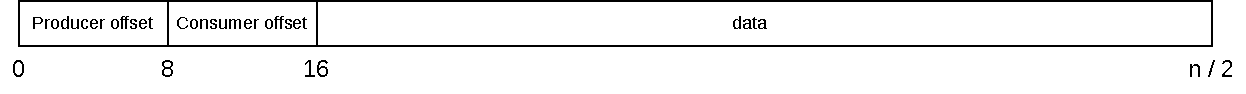
\includegraphics[width=\textwidth, keepaspectratio]{img/circular-buffer-memory.pdf}
    \caption{Memory layout of the circular buffer}
    \label{fig:circular-buffer-memory}
\end{figure}

The mapped memory region is split into 2 equal sections, both containg the same circular buffer data structure. So for a mapped region of size $n$ bytes, and for the start address of the region $s_a$, the second buffer is located on the memory address $s_a + n/2$ ($n$ is always even, as it is a multiple of a page size). Let's denote the start address of a buffer $s_b$

The buffer itself has 2 control variables stored within it. Both are 64-bit unisgned integers representing an offset within the buffers data. The first, located at $s_b$, is the offset at which the producer will write the next chunk of data into the buffer. The second, located at $s_b + 8$, is the offset at which the next chunk of data will be read from the buffer, if present. From the address $s_b + 16$ until the next buffer, or the end of the mapped region, the actual data are stored. That means the actual capacity of data stored within one buffer is $n/2 - 16$.

The data have no uniform size, structure or address alignment. The length of a message in the buffer must be deduced from the data within the message itself. In case of the text encoding, it is the message delimeter. A message can be located at the boundary of the data region. In that case the message is split so that every byte until the very end of the region is filled, and the rest is written at $s_b + 16$ again. There are no gaps between the messages.

The frontend process is responsible for consuming messages from the first buffer and producing them to the second one. As such, the consumer offset of the first buffer and the producer offset of the second buffer must be updated accordingly. The other two offsets must remain read only. The backend process has these roles reversed.



\chapter*{Conclusion}
\addcontentsline{toc}{chapter}{Conclusion}

In the end we managed to develop two nontrivial applications. One for running and simulating the user's Arduino code. The other one for creating a interactive virtual environment, where the Arduino can be connected into a circuit with visual feedback. In chapter \ref{ch:architecture} of this thesis we described the thought process, project structure, and technologies used in order to achieve the goals we set for ourselves in section \ref{sec:goals}. Then we looked into more detail on how we implemented these technologies while avoiding many pitfalls in chapters \ref{ch:backend} and \ref{ch:frontend}.

While we implemented only a couple of most used functions from the Arduino library, and the user interface leaves a lot to be desired, we believe the current version of the product represents a solid foundation on which new functions, events, components and quality of life features can be laid down. One of the biggest hurdles was making sure that the two applications stay synchronized. We succeeded in that regard, by learning a lot of useful information about interprocess communication and approaches commonly used in distributed computing.

A big success also lies in the extensive component system developed in the frontend. The user can extend their component library just by following the specification in section \ref{sec:component_spec}. They can use custom vector graphics, and give life to their components thanks to the abstract \texttt{Component} class. Then they can add it into a scene together with Arduino running their own code. All this while all the heavy work is done by the reflection and parsing machinery on the background. We would be excited to work on this component system, so that it brings even more possibilities to the user.

%%% Bibliography
\include{bibliography}

%%% Figures used in the thesis (consider if this is needed)
\listoffigures

\lstlistoflistings

%%% Tables used in the thesis (consider if this is needed)
%%% In mathematical theses, it could be better to move the list of tables to the beginning of the thesis.
% \listoftables

%%% Abbreviations used in the thesis, if any, including their explanation
%%% In mathematical theses, it could be better to move the list of abbreviations to the beginning of the thesis.
% \chapwithtoc{List of Abbreviations}

%%% Doctoral theses must contain a list of author's publications
\ifx\ThesisType\TypePhD
\chapwithtoc{List of Publications}
\fi

%%% Attachments to the thesis, if any. Each attachment must be referred to
%%% at least once from the text of the thesis. Attachments are numbered.
%%%
%%% The printed version should preferably contain attachments, which can be
%%% read (additional tables and charts, supplementary text, examples of
%%% program output, etc.). The electronic version is more suited for attachments
%%% which will likely be used in an electronic form rather than read (program
%%% source code, data files, interactive charts, etc.). Electronic attachments
%%% should be uploaded to SIS. Allowed file formats are specified in provision
%%% of the rector no. 72/2017. Exceptions can be approved by faculty's coordinator.
\appendix
\chapter{Attachments}

\section{Source code repository} \label{attch:repo}

The file attachment \texttt{thesis.zip} contains the repository with the source code in its entirety. The repository is equivalent with the public git repository found at the URL \url{https://github.com/TenIdiotZInternetu/Arguino} at the tag \xxx{add tag}.

The file structure of the repository is as follows:
\begin{description}
	\item[\texttt{.vscode/}] contains the files:
		\begin{description}
			\item[\texttt{launch.json}] specifies backend debug configurations using the \texttt{cppdbg} VS Code extension.
			\item[\texttt{settings.json}] specifies backend source and build directories using the \texttt{CMakeTools} VS Code extension.
		\end{description}
	\item[\texttt{backend}/] contains the source code for the backend application. Each directory corresponds to a single module described in the chapter \ref{ch:backend}, with the exception of two:
		\begin{description}
			\item[\texttt{libs/}] contains the two utilities modules: \texttt{logger} and \texttt{timer}.
			\item[\texttt{.vscode/}] contains the setup equivalent to the \texttt{.vscode} directory in the root of the repository. 
		\end{description}
		Other files in this directory are:
		\begin{description}
			\item[\texttt{.clang-format}] specification of the automatic code formatting.
			\item[\texttt{.gitignore}] exclusion of build files.
			\item[\texttt{CMakeLists.txt}] main metabuild specification for the backend. References CMake files in the module subdirectories.
			\item[\texttt{CMakePresets.json}] default build configurations using Clang on Linux and MSVC on Windows.
			\item[\texttt{vcpkg.json}] specifies Vcpkg dependencies for the Boost libraries.
			\item[\texttt{preprocess.sh}] shell script performing basic sketch preprocessing using \texttt{arduino-cli}. For use on Linux.
			\item[\texttt{preprocess.bat}] same as \texttt{preprocess.sh} but for the use on Windows. 
		\end{description}
	\item[\texttt{docs/}] Contains year project specification and other documentation:
		\begin{description}
			\item[\texttt{RP\_Specifikacia.odt}, \texttt{RP\_Specifikacia.pdf}] final year project specification in Slovak language.
			\item[\texttt{specification-draft.md}] rough version of the year project specification in English language. Contains the original vision and expectations for the project.
			\item[\texttt{component\_addons\_doc.md}] contains specification of custom components and scenes configuration in the scope of the section \ref{sec:component_spec}.
		\end{description}
	\item[\texttt{frontend/}] contains the source code for the frontend application. Each directory corresponds to a single project described in the chapter \ref{ch:frontend}. The remaining files are \texttt{.gitignore} and the \texttt{gui.sln} .NET solution file.
	\item[\texttt{res/}] contains assets used in source code unrelated context, e.g. screenshots.
	\item[\texttt{tests/}] contains example sketches and scenes used for testing both the frontend and the backend.
	\item[\texttt{thesis/}] contains source files for this document, e.g. \texttt{.tex} files, bibliography files and figures.
	\item[\texttt{.gitignore}] excludes build and Visual Studio files
	\item[\texttt{README.md}] describes the usage and build process of both the backend and the frontend in the scope of the section \ref{sec:usage}.
\end{description}

\end{document}
